\section{Validation}


\subsection{Strategies}
We can emulate a variety of toolpath generation strategies by applying various beading strategies to our framework.

\paragraph{Naive Strategy}


\paragraph{Constant bead count}
Emulates \cite{Ding2016a}


\paragraph{Deviation at middle}
Emulates \cite{Jin2017}


\paragraph{Only outer bead}
Emulates \cite{Moesen2011}


\paragraph{Distributed strategy}
Distribute the overfill or underfill which would happen using a naive strategy over all beads.
This maximizes robustness and minimizes narrow beads qhich are difficult to print.


\paragraph{Combined strategy}
\Cref{wedge_and_infill} shows a combined toolpath strategy.

\begin{figure}
\centering
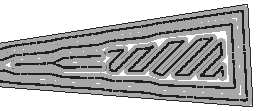
\includegraphics[width=.99\columnwidth]{sources/method/wedge_and_infill.pdf}
\caption{Use single and double wall lines in regions where the infill would be too thin.}
\label{wedge_and_infill}
\end{figure}




\subsection{Filling accuracy}
Render toolpaths and calculate amount of overfilling and amount of underfilling.

\old{Visualize thickness of beads as color.}

Show results for different settings.

\old{Also render with nozzle size as minimal width and use middle of toolpaths instead of middle of beads.}

Example shapes:
\begin{itemize}
\item same as Moessen: grids of triangular holes
\item same as Moessen: circular holes.
\item same as Jin 
\item same as Kao
\item wedge
\item layer of a typical model: phone case
\item some of the above shapes, but with some fuzzy randomized outline
\end{itemize}





\subsection{Experimentation}
Print objects and show qualities:
\begin{itemize}
\item visual consistency of flat top skin surface
\item visual gradual transparency changes
\item graphs of tensile tests on thin walled object
\end{itemize}

Print on mississipi?

What material should I print with for the tensile tests?









